
% This LaTeX was auto-generated from MATLAB code.
% To make changes, update the MATLAB code and republish this document.

\documentclass{article}
\usepackage{graphicx}
\usepackage{color}

\sloppy
\definecolor{lightgray}{gray}{0.5}
\setlength{\parindent}{0pt}

\begin{document}

    
    

\section*{12. Potential theory and approximation}

\begin{verbatim}
ATAPformats
\end{verbatim}
\begin{par}
The explorations of the last chapter are glimmerings of potential theory in the complex plane, a subject that has been connected with approximation of functions since the work of Walsh early in the 20th century [Walsh 1969]. In this chapter we shall outline this connection. Potential theory in the complex plane is presented in [Ransford 1995] and [Finkelshtein 2006], and a survey of applications in approximation theory can be found in [Levin \& Saff 2006].
\end{par} \vspace{1em}
\begin{par}

We begin by looking again at (11.10), the formula giving the ratio of the
size of the node polynomial $\ell$ at an approximation point $x$ to its
size at a point $t$ on a contour $\Gamma$.  Notice that the numerator and
the denominator of this formula each contain a product of $n+1$ terms.
With this in mind, let us define $\gamma_n(x,t)$ as the following
$(n+1)$st root:
$$ \gamma_n(x,t) =
{\left(\prod_{j=0}^n |t-x_j|\right)^{1/(n+1)}  \over
\left( \prod_{j=0}^n |x-x_j|\right)^{1/(n+1)}}. \eqno (12.1) $$
Then the magnitude of the quotient in (11.10) becomes
$$ \left|{\ell(x)\over \ell(t)}\right| = \gamma_n(x,t)^{-n-1}.
\eqno (12.2) $$
This way of writing things brings out a key point: if $\gamma_n(x,t)$ is
bounded above~$1$, we will get exponential convergence as $n\to\infty$.
With this in mind, let us define $\alpha_n$ to be the scalar
$$ \alpha_n = \min_{x\in X,\kern 1pt t\in \Gamma}
\gamma_n(x,t), \eqno (12.3) $$
where $x$ ranges over a domain $X$ where we wish to approximate $f$ (say,
$X=[-1,1]$) and $t$ ranges over a contour $\Gamma$ enclosing that domain.
If $\alpha_n\ge \alpha $ for some $\alpha>1$ for all sufficiently large
$n$, and if $f$ is analytic in the region bounded by $\Gamma$, then
(11.9) tells us that $p(x)$ must converge to $f(x)$ at the rate
$O(\alpha^{-n})$.

\end{par} \vspace{1em}
\begin{par}
 The condition $\alpha_n>1$ has a geometric interpretation.  The
numerator of (12.1) is the geometric mean distance of $t$ to the grid
points $\{x_j\}$, and the denominator is the geometric mean distance of
$x$ to the same points. If $\alpha_n >1$, then every point $t\in\Gamma$
is at least $\alpha_n$ times farther from the grid points, in the
geometric mean sense, than every point $x$ in the approximation domain.
It is this property that allows the Hermite integral formula to show
exponential convergence. 
\end{par} \vspace{1em}
\begin{par}

To bring these observations into potential theory, we linearize the
products by taking logarithms. From (12.1) we find
$$ \log \gamma_n(x,t) =
{1\over n+1} \sum_{j=0}^n \log |t-x_j|-
{1\over n+1} \sum_{j=0}^n \log |x-x_j|. \eqno (12.4) $$
Let us define the {\bf discrete potential function} associated with the
points $x_0,\dots,x_n$ by
$$ u_n(s) = {1\over n+1} \sum_{j=0}^n \log |s-x_j|. \eqno (12.5) $$
Note that $u_n$ is a harmonic function throughout the complex $s$-plane
away from the gridpoints, that is, a solution of the Laplace equation
$\Delta u_n = 0$. We may think of each $x_j$ as a point charge of
strength $1/(n+1)$, like an electron, and of $u_n$ as the potential
generated by all these charges, whose gradient defines an ``electric''
field.  A difference from the electrical case is that whereas electrons
repel one another with an inverse-square force, whose potential function
is inverse-linear, here in the two-dimensional plane the repulsion is
inverse-linear and the potential is logarithmic. (Some authors put a
minus sign in front of (12.5), so that the potential approaches $\infty$
rather than $-\infty$ as $s\to x_j$, making $u_n$ an energy rather than
the negative of an energy.) 
\end{par} \vspace{1em}
\begin{par}

From (12.4) and (12.5) we find
$$ \log\gamma_n(x,t) = u_n(t)-u_n(x), $$
and hence by (12.2),
$$ \left|{\ell(x)\over \ell(t)}\right| = e^{ (n+1)[u_n(x)-u_n(t)]}.
\eqno (12.6) $$
If $\alpha_n\ge \alpha>1$ for all sufficiently large $n$, as considered
above, then $\log \gamma_n(x,t) \ge \log \alpha_n \ge \log \alpha > 0$,
so we have
$$ \min_{t\in \Gamma}u_n(t) - \max_{x\in X} u_n(x) \ge \log\alpha. $$
Together with (11.9) this implies
$$ \|f-p\| = O(e^{-n \log \alpha}). $$
Notice the flavor of this result: the interpolants converge
exponentially, with a convergence constant that depends on the difference
of the values taken by the potential function on the set of points where
the interpolant is to be evaluated and on a contour inside which $f$ is
analytic.

\end{par} \vspace{1em}
\begin{par}

We now take the step from discrete to continuous potentials.
Another way to write (12.5) is as a Lebesgue--Stieltjes integral [Stein \& Shakarchi 2005],
$$ u(s) = \int_{-1}^1 \log |s-\tau| \kern 1pt d \mu(\tau) , \eqno (12.7) $$
where $\mu$ is a measure consisting of a sum of Dirac delta functions,
each of strength $1/(n+1)$,
$$ \mu(\tau) = {1\over n+1} \sum_{j=0}^n \delta(\tau-x_j). \eqno (12.8) $$
This is the {\em potential} or {\em logarithmic potential} associated
with the measure~$\mu$. The same formula (12.7) also applies if $\mu$ is
a continuous measure, which will typically be obtained as the limit of a
family of discrete measures as $n\to\infty$.  (The precise notion of
convergence appropriate for this limit is known as weak* convergence,
pronounced ``weak-star.'') Equally spaced grids in $[-1,1]$ converge to
the limiting measure
$$ \mu(\tau) = {1\over 2}. \eqno (12.9) $$
Chebyshev grids in $[-1,1]$ converge to the
{\em Chebyshev measure} identified in Exercise 2.2,
$$ \mu(\tau) = {1\over \pi \sqrt{1-\tau^2}\kern 1pt}, \eqno (12.10) $$
and so do other grids associated with zeros or extrema of orthogonal
polynomials on $[-1,1]$, such as Legendre, Jacobi, or Gegenbauer
polynomials (see Chapter~17).

\end{par} \vspace{1em}
\begin{par}

And now we can identify the crucial property of the Chebyshev measure
(12.10): {\em The potential\/ $(12.7)$ it generates is constant on}
$[-1,1]$.  The measure is known as the {\em equilibrium measure} for
$[-1,1]$, and physically, it corresponds to one unit of charge adjusting
itself into an equilibrium, minimal-energy distribution.  Given a unit
charge distribution $\mu$ with support on $[-1,1]$, the associated energy
is the integral
$$ I(\mu) = -\int_{-1}^1 u(s) \kern 1ptd \mu(s)
= -\int_{-1}^1 \int_{-1}^1 \log|s-\tau| \kern 1pt d\mu(\tau) \kern 1pt d\mu(s) .
\eqno (12.11) $$
It is clear physically, and can be proved mathematically, that for
$I(\mu)$ to be minimized, $u(s)$ must be constant, so the gradient of the
potential is zero and there are no net forces on the points in $(-1,1)$
[Ransford 1995].

\end{par} \vspace{1em}
\begin{par}
This discussion has gone by speedily, and the reader may have to study these matters several times to appreciate how naturally ideas associated with electric charges connect with the accuracy of polynomial approximations. Potential theory is also of central importance in the study of approximation by rational functions; see [Levin \& Saff 2006] and [Stahl \& Schmelzer 2009].
\end{par} \vspace{1em}
\begin{par}
We have just characterized the equilibrium measure $\mu$ for interpolation on $[-1,1]$ as the unit measure on $[-1,1]$ that generates a potential $u$ that takes a constant value on $[-1,1]$.  To be precise, $u$ is the solution to the following problem involving a Green's function: find a function $u(s)$ in the complex $s$-plane that is harmonic outside $[-1,1]$, approaches a constant value as $s \to [-1,1]$, and is equal to $\log|s| + O(s^{-1})$ as $s\to\infty$. (This last condition comes from the property that the total amount of charge is $1$.) Quite apart from the motivation from approximation theory, suppose we are given this Green's function problem to solve. Since Laplace's equation is invariant under conformal maps, the solution can be derived by introducing a conformal map that transplants the exterior of the interval to the exterior of a disk, taking advantage of the fact that the Green's function problem is trivial on a disk.  Such a mapping is the function $$ z = \phi(s) = {1\over 2} (s + i \sqrt{1-s^2}\kern 1pt), \eqno (12.12) $$ which maps the exterior of $[-1,1]$ in the $s$-plane onto the exterior of the disk $|z|\le 1/2$ in the $z$-plane.  There, the solution of the potential problem is $\log |z|$.  Mapping back to $s$, we find that the Chebyshev potential is given by $u(s) = \log |\phi(s)|$, that is, $$ u(s) = \log |s+i\sqrt{1-s^2}\kern 1pt| - \log 2, \eqno (12.13) $$ with constant value $u(s) = -\log 2$ on $[-1,1]$.
\end{par} \vspace{1em}
\begin{par}
 By definition, the Green's function has a constant
value on $[-1,1]$,
namely $u(s) = -\log 2$.  For values $u_0>-\log 2$, the
equation $u(s) = u_0$ defines an {\em equipotential curve} enclosing
$[-1,1]$ that is
exactly the Bernstein ellipse $E_\rho$ with $\rho = 2\exp(u_0)$, as
defined in Chapter~8. Here is a contour plot of (12.13), confirming that
the contours look the same as the ellipses plotted there. The factor
\verb|sign(imag(s))| is included to make \verb|u| return the correct
branch of the square root for $\hbox{Im}\kern 1pt s < 0$. 
\end{par} \vspace{1em}
\begin{par}
 \vspace{-2em} 
\end{par} \vspace{1em}
\begin{verbatim}
u = @(s) log(abs(s+1i*sign(imag(s)).*sqrt(1-s.^2))) - log(2);
xgrid = -1.5:.02:1.5; ygrid = -0.91:.02:0.91;
[xx,yy] = meshgrid(xgrid,ygrid); ss = xx+1i*yy; uss = u(ss);
levels = -log(2) + log(1.1:0.1:2);
hold off, contour(xgrid,ygrid,uss,levels,'k')
ylim([-0.9,0.9]), axis equal, FS = 'fontsize';
title(['Equipotential curves for the Chebyshev ' ...
            'distribution = Bernstein ellipses'],FS,9)
\end{verbatim}

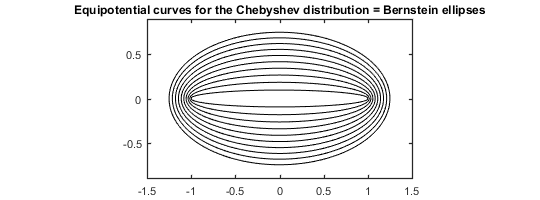
\includegraphics [width=4in]{chap12_01.png}
\begin{par}
 \vspace{1pt} 
\end{par} \vspace{1em}
\begin{par}
The constant ${-}\log 2$ in (12.13) is a reflection of the length of the interval $[-1,1]$.  Specifically, this constant is the logarithm of the \textit{capacity} (or \textit{logarithmic capacity} or \textit{transfinite diameter}) of $[-1,1]$, $$ c = {1\over 2}. $$ The capacity is a standard notion of potential theory, and in a simply connected 2D case like this one, it can be defined as the radius of the equivalent disk. The associated minimal energy is the \textit{Robin constant} of $[-1,1]$: $$ \min_\mu I(\mu) = -\log(c) = \log 2. $$ The fact that the capacity of $[-1,1]$ is $1/2$ has the following interpretation, explored earlier in Exercise 2.6. For Chebyshev or other asymptotically optimal grids on $[-1,1]$, in the limit $n\to\infty$, each grid point lies at a distance $1/2$ from the others in the geometric mean sense.
\end{par} \vspace{1em}
\begin{par}
This is a book about approximation on intervals, but it is worth noting that all these ideas of equilibrium measure, minimal energy, Robin constant and capacity generalize to other compact sets $E$ in the complex plane. If $E$ is connected, then $\mu$ and $u$ can be obtained from a conformal map of its exterior onto the exterior of a disk, whereas if it is disconnected, a more general Green's function problem must be solved. In any case, the equilibrium measure, which is supported on the outer boundary of $E$, describes a good asymptotic distribution of interpolation points as $n\to\infty$, and the limiting geometric mean distance from one point to the others is equal to the capacity, which is related to the Robin constant by $c(E) = \exp(-\min_\mu I(\mu))$.
\end{par} \vspace{1em}
\begin{par}

Having discussed the continuous limit, let us return to the finite
problem of finding good sets of $n+1$ points $\{x_j\}$ for interpolation
by a polynomial $p\in {\cal P}_n$ on a compact set $E$ in the complex
plane. Three particular families of points have received special
attention.  We say that $\{x_j\}$ is a set of {\em Fekete points} for the
given $n$ and $E$ if the quantity
$$ \bigg(\prod_{j\ne k} |x_j-x_k|\bigg)^{2/n(n+1)}, \eqno (12.14) $$
which is the geometric mean of the distances between the points, is as
large as possible, that is, the points are exactly in a minimal-energy
configuration. As $n\to\infty$, these maximal quantities decrease
monotonically to $c(E)$, the fact which gives rise to the expression
``transfinite diameter''. As a rule Fekete points have some of the
cleanest mathematical properties for a given set $E$ but are the hardest
to compute numerically. Next, if $E$ is connected and $\phi(x)$ is a map
of its exterior to the exterior of a disk in the $z$-plane centered at
the origin, a set of {\em Fej\'er points} is a set $\phi^{-1}(\{z_j\})$,
where $\{z_j\}$ consists of any $n+1$ points spaced equally around the
boundary circle.  Fej\'er points are more readily computable since it is
often possible to get one's hands on a suitable mapping $\phi$. Finally,
{\em Leja points} are approximations to Fekete points obtained by a
``greedy algorithm.''  Here, one starts with an arbitrary first point
$x_0\in E$ and then computes successive points $x_1, x_2, \dots$ by an
incremental version of the Fekete condition: with $x_0,\dots , x_{n-1}$
known, $x_n$ is chosen to maximize the same quantity (12.14), or
equivalently, to maximize
$$ \prod_{j=0}^{n-1} |x_j-x_n|. \eqno (12.15) $$
All three of these families of points can be
shown, under reasonable assumptions, to converge to the equilibrium
measure as $n\to\infty$, and all work well in practice for interpolation.
A result showing near-optimality of Leja points for interpolation on
general sets in the complex plane can be found in [Taylor \& Totik 2010].

\end{par} \vspace{1em}
\begin{par}
In Chapter 8 we proved a precise theorem (Theorem 8.2): if $f$ is analytic and bounded by $M$ in the Bernstein ellipse $E_\rho$, then $\|f-p_n\| \le 4M\rho^{-n}/(\kern .5pt \rho-1)$, where $p_n\in {\cal P}_n$ is the interpolant in $n+1$ Chebyshev points.  The proof made use of the Chebyshev expansion of $f$ and the aliasing properties of Chebyshev polynomials at Chebyshev points.  By the methods of potential theory and the Hermite integral formula discussed in this chapter one can derive a much more general theorem to similar effect.  For any set of $n+1$ nodes in $[-1,1]$, let $\ell\in {\cal P}_{n+1}$ be the node polynomial (5.4), and let $M_n = \sup_{x\in[-1,1]} |\ell(x)|$.  A sequence of grids of $1,2,3,\dots$ interpolation nodes is said to be \textit{uniformly distributed} on $[-1,1]$ if it satisfies $$ \lim_{n\to\infty} M_n^{1/n} = {1\over 2}. $$ (On a general set $E$, the number $1/2$ becomes the capacity.)
\end{par} \vspace{1em}
\begin{par}
 \em
{\bf Theorem 12.1. Interpolation in uniformly distributed points.} Given
$f\in C([-1,1])$, let $\rho$ $(1\le \rho \le \infty)$ be the parameter
of the largest Bernstein ellipse $E_\rho$ to which $f$ can be analytically
continued, and let $\{\kern .5pt p_n\}$ be the interpolants to $f$ in any sequence
of grids $\{x_n\}$ of $n+1$ points in $[-1,1]$ uniformly distributed
as defined above. Then the errors satisfy
$$ \lim_{n\to\infty} \| f - p_n \|^{1/n} =\rho^{-1}. \eqno (12.16) $$
\vspace{-1.5em} 
\end{par} \vspace{1em}
\begin{par}
\textit{Proof.} See Chapter 2 of [Gaier 1987]. $~\hbox{\vrule width 2.5pt depth 2.5 pt height 3.5 pt}$
\end{par} \vspace{1em}
\begin{par}
A set of polynomials satisfying (12.16) is said to be \textit{maximally convergent.}  Examples of such polynomials are interpolants through most systems of roots or extrema of Legendre, Chebyshev, or Gauss--Jacobi points; the convergence rates of such systems differ only at the margins, in possible algebraic factors like $n$ or $\log n$.
\end{par} \vspace{1em}
\begin{par}

\begin{displaymath}
\framebox[4.7in][c]{\parbox{4.5in}{\vspace{2pt}\sl
{\sc Summary of Chapter 12.} Polynomial interpolants to analytic
functions on $[-1,1]$ converge geometrically if the grids are asymptotically
distributed according to the Chebyshev distribution.\vspace{2pt}}}
\end{displaymath}

\end{par} \vspace{1em}
\begin{par}
 \small\smallskip\parskip=2pt
\par
{\bf Exercise 12.1.  Fekete points in an interval.}  It can be shown that
the equilibrium configuration for $n+1$ points in $[-1,1]$ consists of
the roots of $(x^2-1) P_{n-1}^{(1,1)}(x)$, where $P_{n-1}^{(1,1)}$ is the
degree $n-1$ Jacobi polynomial with parameters $(1,1)$ [Stieltjes 1885]
(see Chapter~17).
(An equivalent statement is that the points lie at the local extrema in
$[-1,1]$ of the Legendre polynomial of degree $n+1$.)
Thus $(x^2-1) P_{n-1}^{(1,1)}(x)$ is the degree $n-1$ Fekete polynomial
in $[-1,1]$. Verify numerically using the Chebfun {\tt jacpts} command
that in the case $n=10$, the net forces on the 9 interior points are
zero.
\par
{\bf Exercise 12.2.  Capacity of an ellipse.}  Let $E$ be an ellipse
in the complex plane of semiaxis lengths $a$ and $b$.  Show that
$c(E) = (a+b)/2$.
\par
{\bf Exercise 12.3.  Leja points and capacity.}  Let $E$ be
the ``half-moon'' set consisting of the boundary of the right half of the
unit disk.  Write a code to compute a sequence of $100$ Leja points for
this set.  To keep things simple, approximate the boundary by a discrete
set of $1000$ points.  What approximation of the capacity of $E$ do
your points provide?  (The exact answer is $4/3^{3/2}$, as discussed
with other examples and algorithms in [Ransford 2010].)

\end{par} \vspace{1em}



\end{document}
    
